%% LaTeX-Beamer template for KIT design
%% by Erik Burger, Christian Hammer
%% title picture by Klaus Krogmann
%% 
%% version 2.1
%% 
%% mostly compatible to KIT corporate design v2.0
%% http://intranet.kit.edu/gestaltungsrichtlinien.php
%% 
%% Problems, bugs and comments to
%% burger@kit.edu

\documentclass[22pt]{beamer}

%% SLIDE FORMAT

% use 'beamerthemekit' for standard 4:3 ratio
% for widescreen slides (16:9), use 'beamerthemekitwide'

\usepackage{templates/beamerthemekit}
\usepackage[ngerman]{babel}
\usepackage{graphicx}
\usepackage{hyperref}
\usepackage[utf8]{inputenc}
\usepackage{booktabs}
\usepackage{natbib}
\usepackage{bibentry}

\nobibliography*


% \usepackage{templates/beamerthemekitwide}

%% TITLE PICTURE

% if a custom picture is to be used on the title page, copy it into the 'logos'
% directory, in the line below, replace 'mypicture' with the 
% filename (without extension) and uncomment the following line
% (picture proportions: 63 : 20 for standard, 169 : 40 for wide
% *.eps format if you use latex+dvips+ps2pdf, 
% *.jpg/*.png/*.pdf if you use pdflatex)

\titleimage{title2}

%% TITLE LOGO

% for a custom logo on the front page, copy your file into the 'logos'
% directory, insert the filename in the line below and uncomment it

\titlelogo{iosblogo}

% (*.eps format if you use latex+dvips+ps2pdf,
% *.jpg/*.png/*.pdf if you use pdflatex)

%% TikZ INTEGRATION

% use these packages for PCM symbols and UML classes
% \usepackage{templates/tikzkit}
% \usepackage{templates/tikzuml}

% the presentation starts here



\begin{document}

% change the following line to "ngerman" for German style date and logos
\selectlanguage{ngerman}


\date{\today}


\title[#enBW24Hack]{Pitch}

\author{Marvin, Nils, Raphael}

\institute{Case 2}

\begin{frame}

  \titlepage
	
\end{frame}


% table of contents
% \begin{frame}{Gliederung}
%   \tableofcontents[pausesections]
% \end{frame}

% \AtBeginSection[]
% {
% \begin{frame}<beamer>
%   \frametitle{Inhalt}
%   \tableofcontents[currentsection]
% \end{frame}
% }

\section{Konzept}
\subsection{Anforderungen}
    \begin{frame}{Ideen}
    \begin{itemize}
        \item<1-> Datenaufbereitung in dynamischer Geoanwendung
        \item<2-> Individuelle Prognosen und Entscheidungen
        \item<3-> Integration des Userverhaltens
        \item<4-> Intelligentes Assistenzsystem für User + Dispatcher
        \item<5-> Algorithm Trading mit Agenten
    \end{itemize}
    \end{frame}



  \begin{frame}{Überblick}
    \begin{figure}[!h]
      \centering
      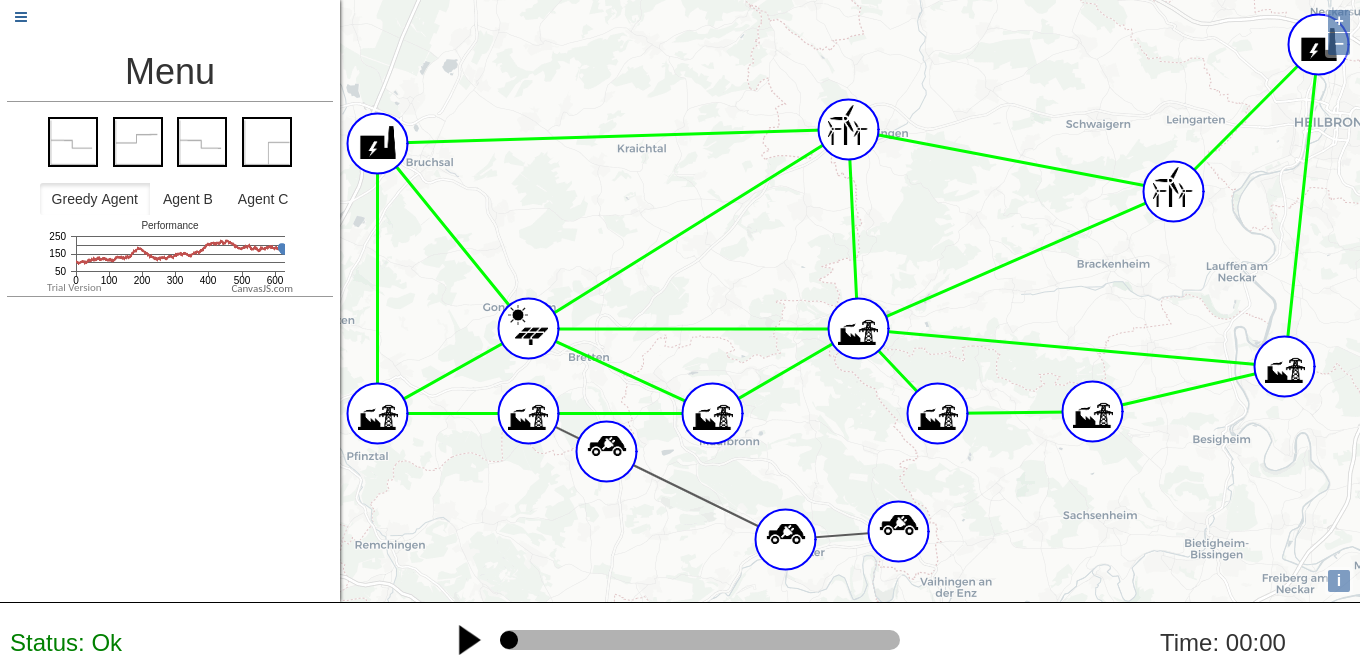
\includegraphics[width=115mm]{resources/overview.png}
      \label{fig:overview}
    \end{figure}
	\end{frame}

\begin{frame}{Dispatcher und User Agenten}
    \begin{figure}[!h]
      \centering
      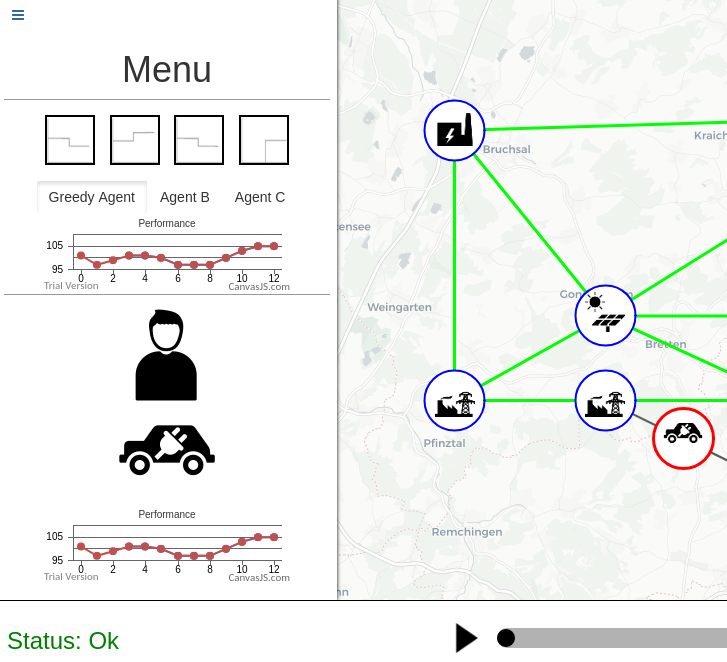
\includegraphics[width=80mm]{resources/enduser.png}
      \label{fig:projectplan}
    \end{figure}
  \end{frame}
  \begin{frame}{Detailinformationen}
    \begin{figure}[!h]
      \centering
      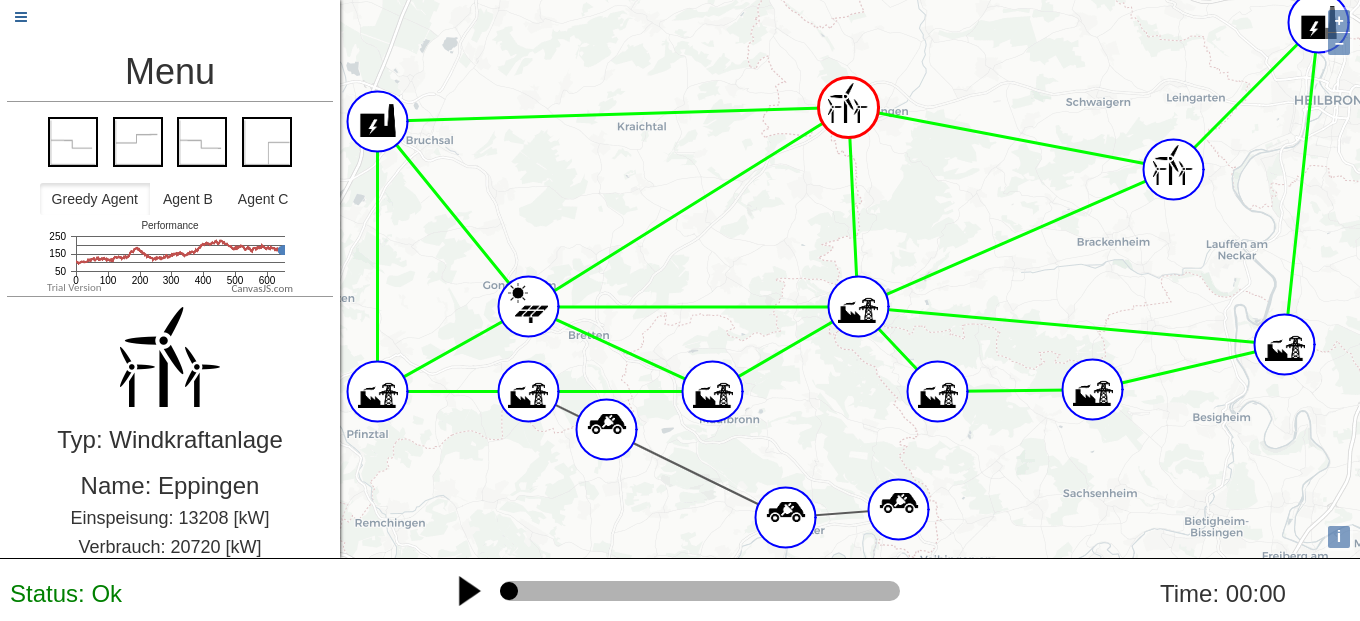
\includegraphics[width=115mm]{resources/selected.png}
      \label{fig:projectplan}
    \end{figure}
\end{frame}

\begin{frame}{Fluss Berechnung}
    \begin{figure}[!h]
      \centering
      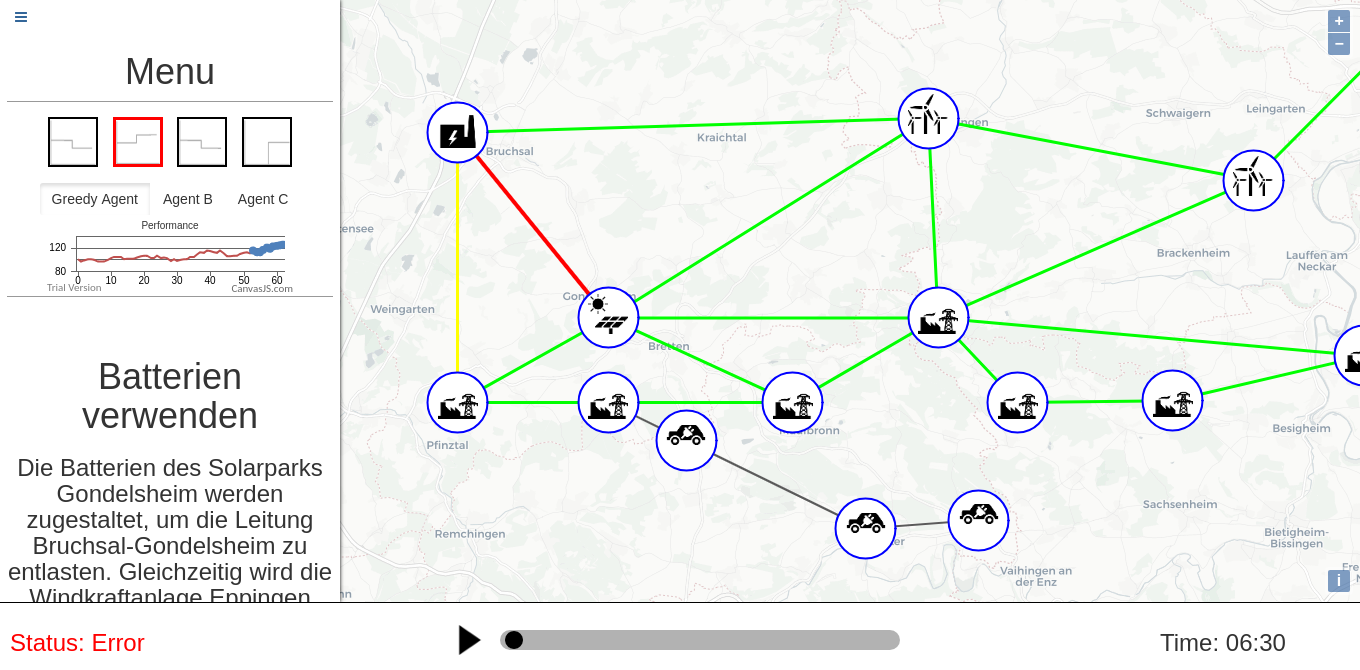
\includegraphics[width=115mm]{resources/action.png}
      \label{fig:projectplan}
    \end{figure}
  \end{frame}
  
\begin{frame}{Fehlerbehebung}
    \begin{figure}[!h]
      \centering
      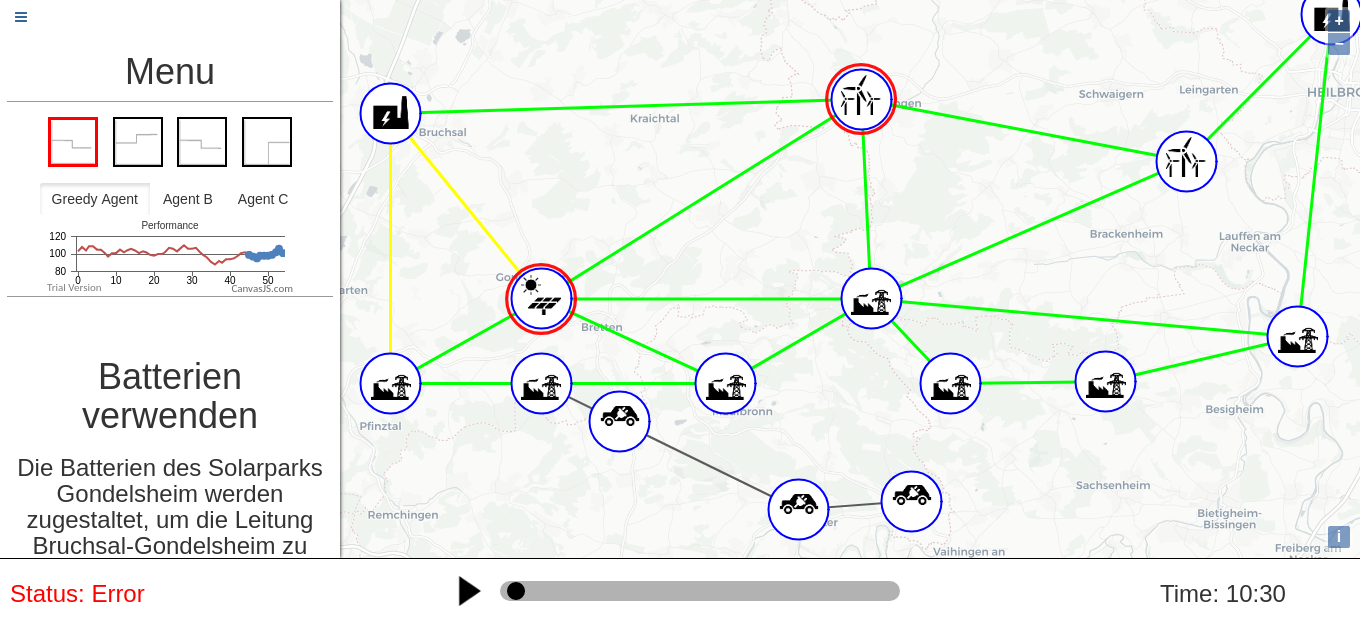
\includegraphics[width=115mm]{resources/mark.png}
      \label{fig:projectplan}
    \end{figure}
\end{frame}

\bibliographystyle{plain}

\begin{frame}{References}
  \bibliography{../References/references}
\end{frame}


\end{document}
